\documentclass[aspectratio=169]{beamer}

\usepackage[utf8]{inputenc}

\usepackage{amsfonts}
\usepackage{amsmath}
\usepackage{color}
\usepackage{listings}
\usepackage{tikz}
\usepackage{hyperref}

\usetheme{Rochester}
\usecolortheme{beaver}

\addtobeamertemplate{navigation symbols}{}{%
    \usebeamerfont{footline}%
    \usebeamercolor[fg]{footline}%
    \hspace{1em}%
    \insertframenumber/\inserttotalframenumber
}

\lstloadlanguages{C++}
    \lstset{%
        language={C++},
        basicstyle=\ttfamily,
        keywordstyle=\color{blue},
        showstringspaces=false,
        escapechar={§},
        escapeinside=||
    }

\newif\iftransitions
 \transitionstrue


\newif\iffast
% \fasttrue

\title{Exceptions Demystified}
% \subtitle{An Introduction to Custom Allocators}
\author{Andreas Weis}
\institute{BMW AG}

\date{MUC++, April 25, 2019}
%\titlegraphic{
\includegraphics[height=.15\textheight]{resources/accu2019_logo.png}}

\iffalse
Exceptions Demystified

Exception Handling is probably one of the most controversial features in C++, with many code bases outright banning them from the start, or only allowing their use in very specific cases. The reasons for this are often unclear and founded on premises that are not well understood.

In this talk, we will explain exception handling from the bottom up, taking a close look at what a compiler actually has to do to implement the mechanism. Instead of focusing on a specific implementation, we will approach the problem from a more abstract, language-design point of view, allowing us to explore the different approaches an implementation could choose. In the end, we will gain a deeper understanding for the problems associated with the feature and how they could be mitigated in the future by alternative language features like the proposed static exceptions.


Audience
Language users familiar with exceptions, but not with the underlying implementation

Outline
- Lifetime of an exception
- Anatomy of the call stack
- Finding the right catch
- RTTI
- Unwinding the stack
- Exceptions in restricted environments (real-time, embedded)
- Execution time analysis in the presence of exceptions
- Alternative mechanisms (static exceptions)

Video
https://www.youtube.com/watch?v=S7I66lZX_zM
https://www.youtube.com/watch?v=FcpmMmyNNv8
https://www.youtube.com/watch?v=_8vMAkCp0Rc

Comments
This talk is similar in spirit to Dave Watson's CppCon 2017 talk (https://www.youtube.com/watch?v=_Ivd3qzgT7U) or James McNellis' CppCon 2018 talk (https://www.youtube.com/watch?v=COEv2kq_Ht8). Unlike those, I don't want to focus on a specific implementation, but explain the underlying algorithmic problems that these implementations want to solve. The focus here will also be very much on how those influence the life of an application developer and hopefully separate the valid concerns about exceptions as a feature from the FUD.
\fi

\begin{document}

\frame{\titlepage}

\iftrue %crop

\begin{frame}[fragile]
  \frametitle{About me}

  \begin{itemize}
    \setlength\itemsep{1.5em}

    \item \href{https://stackoverflow.com/users/577603/comicsansms}{
\includegraphics[height=.05\textheight]{resources/so-icon.png}} \href{https://github.com/ComicSansMS}{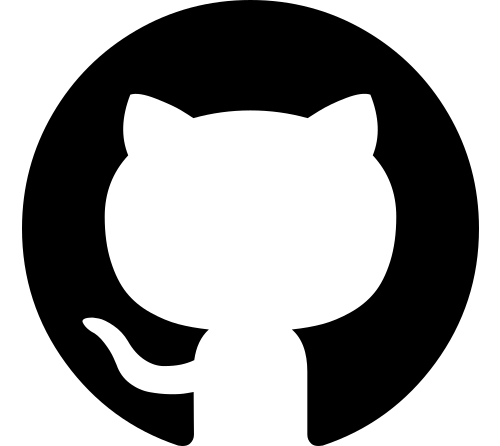
\includegraphics[height=.05\textheight]{resources/github-icon.png}} 
\includegraphics[height=.05\textheight]{resources/slack-icon.png} ComicSansMS

    \item \href{https://twitter.com/DerGhulbus/}{
\includegraphics[height=.05\textheight]{resources/twitter-icon.png} @DerGhulbus}

    \item 
\includegraphics[height=.05\textheight]{resources/meetup-icon.png} Co-organizer of the \href{https://www.meetup.com/MUCplusplus/}{Munich C++ User Group}

    \item Currently working as a Software Architect for BMW 
\includegraphics[height=.1\textheight]{resources/bmw_group.jpg}

  \end{itemize}
\end{frame}


\begin{frame}
  \frametitle{Overview}
  \begin{itemize}
  \item Lifetime of an exception
  \item Anatomy of the call stack
  \item Finding the right catch
  \item RTTI
  \item Unwinding the stack
  \item Exceptions in restricted environments (real-time, embedded)
  \item Execution time analysis in the presence of exceptions
  \item Alternative mechanisms (static exceptions)
  \end{itemize}
\end{frame}

\begin{frame}[fragile]
  \frametitle{Lifetime of an exception}
  \begin{lstlisting}[language={C++}]
void f() {
    throw MyException{};  // starts here      
}

void g() {
  try {
    f();
  } catch(MyException& e) {
    // dies here
  }
}
  \end{lstlisting}
\end{frame}

\begin{frame}[fragile]
  \frametitle{Lifetime of an exception}
  \begin{lstlisting}[language={C++}]
void f() {
    throw MyException{};  // starts here      
}

std::exception_ptr g_exc;

void g() {
  try {
    f();
  } catch(...) {
    g_exc = std::current_exception();
  }
}
  \end{lstlisting}
\end{frame}

\begin{frame}[fragile]
  \frametitle{Lifetime of an exception}
  \begin{lstlisting}[language={C++}]
void f() {
    throw MyException{};  // starts here      
}

std::vector<std::exception_ptr> g_excs;

void g() {
  try {
    f();
  } catch(...) {
    g_excs.push_back(std::current_exception());
  }
}
  \end{lstlisting}
\end{frame}

\begin{frame}
  \frametitle{Responsibilities of \texttt{throw}}

  \begin{itemize}
  \item Create the exception object
    \begin{itemize}
    \item Memory for the exception is allocated in an unspecified way [except.throw]
    \item As a consequence, there is no official customization point for this allocation
    \item Many implementations today simply perform a heap allocation
    \end{itemize}
  \item Transfer control to the exception handler
    \begin{itemize}
    \item The standard does not mention how this transfer of control is achieved
    \item It does mandate though, that destructors must be invoked for objects along the path from \texttt{throw} to the handler $\Rightarrow$ \emph{stack unwinding} [except.ctor]
    \end{itemize}
  \end{itemize}
\end{frame}

\begin{frame}
  \frametitle{Storage of the exception object}

  \begin{itemize}
  \item Exception objects can be of arbitrary size. Allocate on the heap?
  \item \texttt{std::bad\_alloc} is a common exception
  \item Stack?
  \item We still need to perform calls to destructors during unwinding (each of which can have their own, nested exceptions)
  \item Since C++11, an exception can outlive the handler (\texttt{exception\_ptr}), so these for sure cannot be left on the stack
  \end{itemize}
\end{frame}

\begin{frame}
  \frametitle{Customizing storage of the exception object}
  \begin{itemize}
  \item Most implementations today simply invoke malloc for allocating storage for the exception object
  \item Replacing malloc can be an option for certain scenarios
  \item Is it a problem to allocate exceptions from a fixed-size arena? It might be, as that turns each \texttt{throw} and \texttt{exception\_ptr} use into a potential \texttt{terminate}
  \item In practice, we already have a similar situation today with \texttt{bad\_alloc}
  \end{itemize}
\end{frame}

% Exception_ptr & Stack of Exceptions
% throw as terminate

\begin{frame}
  \frametitle{Anatomy of the call stack}

  \begin{columns}
    \begin{column}{.5\textwidth}
      \includegraphics<1>[height=.95\textheight]{excgfx/stack_010.png}
      \includegraphics<2>[height=.95\textheight]{excgfx/stack_020.png}
      \includegraphics<3>[height=.95\textheight]{excgfx/stack_030.png}
      \includegraphics<4>[height=.95\textheight]{excgfx/stack_040.png}
      \includegraphics<5>[height=.95\textheight]{excgfx/stack_050.png}
      \includegraphics<6>[height=.95\textheight]{excgfx/stack_060.png}
      \includegraphics<7>[height=.95\textheight]{excgfx/stack_070.png}
      \includegraphics<8>[height=.95\textheight]{excgfx/stack_080.png}
      \includegraphics<9>[height=.95\textheight]{excgfx/stack_090.png}
    \end{column}
    
    \begin{column}{.5\textwidth}
      \begin{center}
        Lorem ipsum

        Solor domit

        Bli bla blub
      \end{center}
    \end{column}
  \end{columns}

\end{frame}



\begin{frame}
  \frametitle{Thanks for your attention.}

  \href{https://stackoverflow.com/users/577603/comicsansms}{
\includegraphics[height=.05\textheight]{resources/so-icon.png}}
  \href{https://github.com/ComicSansMS}{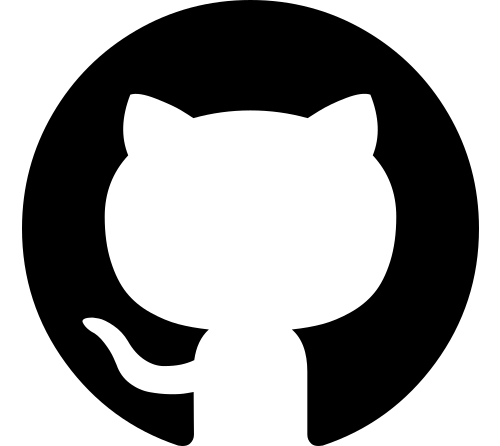
\includegraphics[height=.05\textheight]{resources/github-icon.png}}
  
\includegraphics[height=.05\textheight]{resources/slack-icon.png} ComicSansMS /
  \href{https://twitter.com/DerGhulbus/}{
\includegraphics[height=.05\textheight]{resources/twitter-icon.png} @DerGhulbus}

\end{frame}


\end{document}
